% !TeX encoding = UTF-8
% !TeX spellcheck = en_US

\chapter{Fluid-dynamic Equations}
\label{chap:macroscopic}


The derivation of macroscopic equations in closed forms from the Boltzmann equation is of both fundamental and practical importance, since the structure of Boltzmann collision operator is complicated and difficult to handle both theoretically and numerically. And there are huge demanding of macroscopic equations that allow efficient and accurate calculation of rarefied gas dynamics with applications from aerodynamics to microfludics. It has also been considered as an important part in the sixth Hilbert problem: ``Thus Boltzmann's work on the principles of mechanics suggests the problem of developing mathematically the limiting processes, which lead from the atomistic view to the laws of motion of continua''~\cite{Hilbert1902}. In this Chapter we first introduce how macroscopic equations are derived, and then assess the their accuracy. % in the problems of Rayleigh-Brillouin scattering and sound wave damping. 


\section{Hilbert expansion}

Macroscopic equations like Eq.~\eqref{macro} can be obtained by multiplying the Boltzmann equation~\eqref{Boltzmann} with the collision invariants and integrating with respect to the molecular velocity $\bm{v}$. However, the obtained moment system is not closed because expressions for the stress and heat flux are not known. Hilbert proposed to solve the Boltzmann equation via a formal asymptotic expansion of the VDF as~\cite{Hilbert1912}:
\begin{equation}\label{asymptotic}
f(t,\bm{x},\bm{v})=\sum_{n=0}^\infty {\epsilon^n} f^{(n)}(t,\bm{x},\bm{v}),
\end{equation}
where $\epsilon$ is a formal small parameter which plays the role of spatial Knudsen number for monitoring the order of terms and quantities appearing in the equations, which will be replaced by one when the solutions are obtained. Meanwhile, the Boltzmann collision operator is written as
\begin{equation}
\frac{Q}{\epsilon}=\sum_{n=0}^\infty {\epsilon^{n-1}} Q^{(n)}, 
\end{equation} 
where $Q^{(0)}=Q(f^{(0)},f^{(0)})$ and $Q^{(1)}=f^{(0)}\mathcal{J}(\phi)$ if we write $f^{(1)}=f^{(0)}\phi$.

The macroscopic variables are also expressed into the power series of $\epsilon$ according to Eq.~\eqref{macroscopic_origin}:
\begin{equation}\label{conservative_hilbert}
\begin{aligned}[b]
\left[\rho,\rho\bm{u},\frac{3}{2}k_B\rho{}T\right]=\sum_{n=0}^\infty \epsilon^n \int \left[1,\bm{v}, \frac{1}{2}mc^2\right]mf^{(n)}d\bm{v},
\end{aligned}
\end{equation} 
and
\begin{equation}\label{shere_hilbert}
\begin{aligned}[b]
p_{ij} &=\sum_{n=0}^\infty \epsilon^n p_{ij}^{(n)},
\quad
p^{(n)}_{ij}=\int{}mc_ic_jf^{(n)}d\bm{v}
 \\  
 \bm{q} &=\sum_{n=0}^\infty \epsilon^n \bm{q}^{(n)}, 
 \quad
 \bm{q}^{(n)}=\int{}\frac{1}{2}mc^2\bm{c}f^{(n)}d\bm{v}.
 \end{aligned}
\end{equation}

Substituting Eq.~\eqref{asymptotic} into the Boltzmann equation and collecting powers of $\epsilon$ yields an infinite system of integro-differential equations for $f^{(n)}$. At the order $O(\epsilon^{-1})$ we have $Q^{(0)}=0$.
Therefore, $f^{(0)}$ is the equilibrium distribution function~\eqref{equilibrium_Maxwellian}:
\begin{equation}
f^{(0)}
=\frac{\rho^{(0)}}{m}\left(\frac{m}{2\pi   k_BT^{(0)}}\right)^{3/2}\exp\left(-\frac{m(\bm{v}-\bm{u}^{(0)})^2}{2k_BT^{(0)}}\right),
\end{equation}
but the density, velocity and temperature are evaluated at the zeroth-order expansion, e.g., $\rho^{(0)}=\int {mf^{(0)}d\bm{v}}$. 
If only this zeroth-order expansion is adopted, we have  $\rho^{(0)}=\rho$, $\bm{u}^{(0)}=\bm{u}$, and $T^{(0)}=T$. Therefore, the corresponding set of macroscopic equations are the Euler equations, i.e., Eq.~\eqref{macro} with
$p_{ij}=nk_BT\delta_{ij}$ and $\bm{q}=0$. When the first-order expansion in VDF is considered: $f=f^{(0)}+f^{(0)}\phi$, we have 
\begin{equation}\label{Q1_Hilbert}
f^{(0)}\mathcal{J}(\phi)= 
\frac{\partial f^{(0)}}{\partial t}+\bm{v}\cdot\frac{\partial f^{(0)}}{\partial
	\bm{x}}+\bm{a}\cdot\frac{\partial f^{(0)}}{\partial \bm{v}}.
\end{equation}
%In this case, $f^{(0)}$ is still given by the equilibrium VDF $F_{eq}$,
By solving Eq.~\eqref{Q1_Hilbert}, one can obtain $\phi$ and hence $f^{(1)}$; and the process can be carried on to obtain high-order approximations. We refer to the monograph of Sone~\cite{Sone2002Book} for more details. However, it should be noted that the NSF equations never emerge according to the Hilbert expansion.



\section{Chapman-Enskog expansion}\label{Champan_Enskog_expansion}
\index{Chapman-Enskog expansion}
\index{Chapman-Enskog expansion!Navier-Stokes-Fourier equations}

Chapman and Enskog independently proposed a new technique~\cite{Chapman1916,Enskog1917}, which has become the standard procedure to derive macroscopic equations from the kinetic equation. The most successful part is that the transport coefficients in NSF equations can be derived as long as the intermolecular potential is known. In the Chapman-Enskog expansion, the VDF, stress and heat flux remain the same as the Hilbert expansion. However, the five conservative variables $C_M=\{\rho,\bm{u}, T\}$  are calculated only according to the zeroth-order expansion. That is, 
\begin{eqnarray}\label{density_hilbert}
\left[\rho,\rho\bm{u},\frac{3}{2}k_B\rho{}T\right]=
m\int{}\left[1,\bm{v},\frac{1}{2}mc^2\right]f^{(0)}d\bm{v},  
\end{eqnarray}
with the compatibility condition
\begin{eqnarray} \label{compatibility}
\int{}f^{(n)}d\bm{v}=\int{}\bm{v}f^{(n)}d\bm{v}=\int{}c^2f^{(n)}d\bm{v}=0, \quad \text{for} \quad n\ge1.
\end{eqnarray}


On substituting the above equations to Eq.~\eqref{macro}, one finds that the time derivatives is formally written as a series in $\epsilon$~\cite{henning}:
\begin{equation}\label{fast_slow_time}
\frac{\partial}{\partial{} t}=\sum_{n=0}^\infty \epsilon^n \frac{\partial}{\partial{} t_n}.
\end{equation}
Therefore, at the zeroth-order approximation, we have
\begin{equation}\label{eq123_zerothOrder}
\begin{aligned}[b]
\frac{\partial \rho}{\partial t_0}+\frac{\partial(\rho{}u_j) }{\partial x_j}=0, \\
\frac{\partial (\rho{u_i})}{\partial t_0}+\frac{\partial (\rho{}u_iu_j+nk_BT\delta_{ij})}{\partial x_j}= \rho{}a_i,\\
\frac{\partial \left(\rho{}E\right)}{\partial t_0}+\frac{\partial \left(\rho{}{E}u_j+u_ink_BT\delta_{ij}\right)}{\partial x_j}=\rho{}a_ju_j,
\end{aligned}
\end{equation} 
while at other orders $(n>0)$ we have
\begin{equation}\label{eq123_HighOrder}
\begin{aligned}[b]
\frac{\partial \rho}{\partial t_n}=0, \quad
\frac{\partial (\rho{u_i})}{\partial t_n}+\frac{\partial p^{(n)}_{ij}}{\partial x_j}= 0,\quad
\frac{\partial \left(\rho{}E\right)}{\partial t_n}+\frac{\partial \left(u_ip^{(n)}_{ij}+q^{(n)}_j\right)}{\partial x_j}=0.
\end{aligned}
\end{equation} 

%The Maxwellian $F_{eq}$ depends on the conservative variables and the above expansion can be used to expand its time derivative according to 
%\begin{equation}
%\frac{DF_{eq}}{Dt}=\frac{DF_{eq}}{Dt_0}+\epsilon\frac{DF_{eq}}{Dt_1}+\cdots,
%\end{equation}
%where 
%\begin{equation}
%\frac{DF_{eq}}{Dt_\epsilon}=
%\frac{\partial F_{eq}}{\partial C_M}
%\frac{\partial C_M}{\partial t_\epsilon}.
%\end{equation}


%\subsection{Transport coefficients}
\index{transport coefficient}
\index{shear viscosity}
\index{thermal conductivity}


At the order $O(\epsilon^{-1})$, like the Hilbert expansion, we have $Q(f^{(0)},f^{(0)})=0$. Hence $f^{(0)}$ is just the equilibrium distribution function~\eqref{equilibrium_Maxwellian}, because the conservative variables $C_M$ are determined only according to the zeroth-order expansion. 

At the order $O(1)$, the VDF $f^{(1)}=F_{eq}\phi$ satisfies the following equation:
\begin{equation}\label{integral_solution}
\begin{aligned}[b]
F_{eq}\mathcal{J}(\phi)=&\frac{\partial F_{eq}}{\partial t_0}+\bm{v}\cdot\frac{\partial F_{eq}}{\partial
	\bm{x}}+\bm{a}\cdot\frac{\partial F_{eq}}{\partial \bm{v}}\\
=&\left[
2\xi_{\langle{i}} \xi_{j\rangle}
\frac{\partial u_{\langle{i}}}{\partial x_{j\rangle}}
+\left(\xi^2-\frac{5}{2}\right)\xi_i\sqrt{\frac{2k_BT}{m}}\frac{\partial \ln{T}}{\partial x_i}
\right]F_{eq}.
\end{aligned}
\end{equation}
Note that the final equation is obtained with the help of $\frac{\partial F_{eq}}{\partial t_0}=
\frac{\partial F_{eq}}{\partial C_M}
\frac{\partial C_M}{\partial t_0}$,  $\frac{\partial F_{eq}}{\partial \bm{x}}=
\frac{\partial F_{eq}}{\partial C_M}
\frac{\partial C_M}{\partial \bm{x}}$, and Eq.~\eqref{eq123_zerothOrder}. Details can be found in Struchtrup's book~\cite{henning}.

The solution of the integral equation~\eqref{integral_solution} can be decomposed into a homogeneous part and inhomogeneous part. The homogeneous part of solution satisfied $\mathcal{J}(\phi)=0$, thus $\phi$ must be linear combinations of collisional invariants. However, the compatibility condition~\eqref{compatibility} requires that all the combination coefficients are zero. The inhomogeneous solution must be read
\begin{equation}
\phi=
-A_\mu(\xi)\xi_{\langle{i}} \xi_{j\rangle}\frac{\partial u_{\langle{i}}}{\partial x_{j\rangle}}
-A_\kappa(\xi)\xi_i\sqrt{\frac{2k_BT}{m}}\frac{\partial \ln{T}}{\partial x_i},
\end{equation}
where $\int \xi^2A_\kappa(\xi)F_{eq}d\bm{v}=0$ for the compatibility condition~\eqref{compatibility}, and the solutions of $A_\kappa(\xi)$ and $A_\mu(\xi)$ satisfy
\begin{equation}\label{transport_coefficient_0}
\begin{aligned}[b]
\mathcal{J}(A_\mu\xi_{\langle{i}} \xi_{j\rangle})&=-2\xi_{\langle{i}} \xi_{j\rangle},
\text{~and~}
\mathcal{J}(A_\kappa\xi_i)&=-\left(\xi^2-\frac{5}{2}\right)\xi_i.
\end{aligned}
\end{equation}


Once $A_\kappa(\xi)$ and $A_\mu(\xi)$ are known, Newton's law for stress and Fourier's law for heat conduction can be obtained:
\begin{equation}
\begin{aligned}[b]
\sigma^{(1)}_{ij}=-2\mu\frac{\partial u_{\langle i}}{\partial x_{j\rangle}},
\text{~and~}
q^{(1)}_i=-\kappa \frac{\partial T}{\partial x_i},
\end{aligned}
\end{equation} where the shear viscosity and heat conductivity are
\begin{equation}\label{viscosity_original}
\begin{aligned}[b]
\mu=&\frac{2p}{15\pi^{3/2}}\int\exp(-\xi^2)A_\mu(\xi)\xi^4d\bm{\xi},
\\
\kappa=&\frac{2p}{3\pi^{3/2}}
\frac{k_B}{m}
\int\exp(-\xi^2)A_\kappa(\xi)\xi^4
d\bm{\xi}.
\end{aligned}
\end{equation}

The NSF equations are obtained by combining Eqs.~\eqref{fast_slow_time}, \eqref{eq123_zerothOrder} and \eqref{eq123_HighOrder} with $n=1$, which is accurate to $O(\text{Kn})$. 


%\subsubsection{Variational solution}

\subsubsection{Expansion in Sonine polynomials}

Although Eq.~\eqref{transport_coefficient_0} can be solved exactly by the fast spectral method so that the transport coefficients in Eq.~\eqref{viscosity_original} can be calculated exactly (see Section~\ref{accurate_transport}), an analytical derivation will be beneficial. 

With the Sonine polynomials in Appendix~\ref{appendix_special_functions}, the integral equation~\eqref{transport_coefficient_0} can be written as $\mathcal{J}(A_\kappa\xi_i)=S^{(1)}_{\frac{3}{2}}(\xi^2)\xi_i$ and $\mathcal{J}(A_\mu\xi_{\langle{i}}\xi_{j\rangle})=-2S^{(0)}_{\frac{5}{2}}(\xi^2) \xi_{\langle{i}}\xi_{j\rangle}$. For their solution, $A_\kappa(\xi)$ and $A_\mu(\xi)$ are expanded as
\begin{equation}\label{sonine_expansion}
\begin{aligned}[b]
A_\kappa(\xi)=-\sum_{r=1}^{n_a}a_rS^{(r)}_{\frac{3}{2}}(\xi^2), 
\text{~and~}
A_\mu(\xi)=\sum_{r=0}^{n_b}b_rS^{(r)}_{\frac{5}{2}}(\xi^2).
\end{aligned}
\end{equation}





Multiplying Eq.~\eqref{transport_coefficient_0} with $\exp(-\xi^2)S^{(s)}_{\frac{3}{2}}(\xi^2)\xi_i$ and $\exp(-\xi^2)S^{(s)}_{\frac{5}{2}}(\xi^2)\xi_{\langle{i}}\xi_{j\rangle}$, respectively, and  taking advantage of the orthogonality of Sonine's polynomials, we have
\begin{equation}
\begin{aligned}[b]
&\sum_{r=1}^{n_a}\alpha_{sr}a_r=\frac{15}{4}\pi^3\frac{m}{\rho}\delta_{s1}, \quad
&\sum_{r=1}^{n_a}\beta_{sr}b_r=5\pi^3\frac{m}{\rho}\delta_{s0},
\end{aligned}
\end{equation} 
%\begin{equation}
%\begin{aligned}[b]
%&\sum_{r=1}^{n_a}\alpha_{sr}a_r=\frac{15}{4}\pi^3\frac{m}{\rho}\delta_{s1} \Longrightarrow
%a_r=\frac{15}{4}\pi^3\frac{m}{\rho}\alpha^{-1}_{r1},\\
%&\sum_{r=1}^{n_a}\beta_{sr}b_r=5\pi^3\frac{m}{\rho}\delta_{s0} \Longrightarrow
%b_r=5\pi^3\frac{m}{\rho}\beta^{-1}_{r0},
%\end{aligned}
%\end{equation} 
where the matrices $\alpha_{sr}$ and $\beta_{sr}$ are
\begin{equation}
\begin{aligned}[b]
\alpha_{sr}=\left[S^{(s)}_{\frac{3}{2}}(\xi^2)\xi_i,S^{(r)}_{\frac{3}{2}}(\xi^2)\xi_i\right],\quad
\beta_{sr}=\left[S^{(s)}_{\frac{5}{2}}(\xi^2)\xi_{\langle{i}}\xi_{j\rangle},S^{(r)}_{\frac{5}{2}}(\xi^2)\xi_{\langle{i}}\xi_{j\rangle}\right],
\end{aligned}
\end{equation}
with the bracket operator defined in Eq.~\eqref{integral_equation}.

Note that with the compatibility equation the last equation in Eq.~\eqref{viscosity_original} can be rewritten as
	$
	\kappa=\frac{2p}{3\pi^{3/2}}
	\frac{k_B}{m}
	\int\exp(-\xi^2)A_\kappa(\xi)\xi_i
	\left(\xi^2-\frac{5}{2}\right)
	\xi_i
	d\bm{\xi}$.
Therefore, together with Eq.~\eqref{sonine_expansion}, we have
\begin{equation}\label{viscosity_general_fundamental}
\mu=\frac{p}{2}b_0, 
\quad
\kappa=\frac{p}{2}a_1.
\end{equation}
In order to obtain the analytical expressions for shear viscosity and thermal conductivity, we need to compute $\alpha_{sr}$ and $\beta_{sr}$, and their inverses. %from which we only require the elements $\alpha^{-1}_{11}$ and $\beta^{-1}_{00}$
Their values depend on the numbers of $n_a$ and $n_b$ in Eq.~\eqref{sonine_expansion}. However, for Maxwell molecules, according to Eq.~\eqref{Wang_Chang}, $\alpha_{sr}$ and $\beta_{sr}$ are diagonal, so 
%$\alpha^{-1}_{11}=1/\alpha_{11}$ and $\beta^{-1}_{00}=1/\beta_{00}$.
\begin{equation}\label{viscosity_general}
\mu=\frac{p}{2}b_0=\frac{5\pi^3}{2}k_BT\beta^{-1}_{00}, 
\quad
\kappa=\frac{p}{2}a_1=\frac{75\pi^3}{8}\frac{k_B}{m}k_BT\alpha^{-1}_{11}.
\end{equation}
For other intermolecular potentials, this approximation already give a very accurate estimation of the transport coefficients, as we will see immediately below.





\subsubsection{Expansion to the first-order}


If only one element in each expansion in Eq.~\eqref{sonine_expansion} is used, we get 
\begin{equation}\label{alpha_beta}
\begin{aligned}[b]
\alpha_{11}
=&\frac{1}{4}\int \exp(-\xi^2-\xi^2_\ast)
\mathcal{D}^2(\xi^2\xi_i)B(\cos\theta,v_r)d\Omega{d\bm{\xi}_\ast}d\bm{\xi},\\
\beta_{00}=&\frac{1}{4}\int \exp(-\xi^2-\xi^2_\ast)
\mathcal{D}^2(\xi_{\langle{i}}\xi_{j\rangle})
B(\cos\theta,v_r)
d\Omega{d\bm{\xi}_\ast}d\bm{\xi},
\end{aligned}
\end{equation}
where $\mathcal{D}(\psi)=\psi+\psi_\ast-\psi'-\psi'_\ast$. 

If we define $\eta_i=\xi_i-\xi_{\ast {i}}$, 
$\zeta_i=\frac{1}{2}(\xi_i+\xi_{\ast {i}})=\frac{1}{2}(\xi'_i+\xi'_{\ast {i}})$,  $\eta'_i=\xi'_i-\xi'_{\ast {i}}$, 
 and $v_r=v_m\eta$, we have $\xi^2+\xi^2_{\ast}=2\zeta^2+\frac{1}{2}\eta^2$, ${d\bm{\xi}_\ast}d\bm{\xi}=d\bm{\eta}d\bm{\zeta}$,
${D}(\xi^2\xi_i)=\zeta_i(\eta_i\eta_j-\eta'_i\eta'_j)$, 
$\mathcal{D}(\xi_{\langle{i}}\xi_{j\rangle})=\frac{1}{2}(\eta_i\eta_j-\eta'_i\eta'_j)$. Thus,
\begin{equation*}
\begin{aligned}[b]
\mathcal{D}^2(\xi_{\langle{i}}\xi_{j\rangle})=&\frac{1}{4}(\eta_i\eta_j-\eta'_i\eta'_j)(\eta_i\eta_j-\eta'_i\eta'_j)\\
=&\frac{1}{2}(\eta^4-\eta_i\eta'_i\eta_j\eta'_j)=\frac{1}{2}\eta^4\sin^2\theta,
\end{aligned}
\end{equation*} 
where the last equation is obtained by the fact that the relative velocity is deflected by an angle of $\theta$ after the binary collision, while its magnitude remains unchanged, see Fig.~\ref{Boltzmann_collision_demo}. 


In the calculation of ${D}^2(\xi^2\xi_i)$, if we ignore the terms which have zero contribution to the integral in Eq.~\eqref{alpha_beta}, we have
\begin{equation*}
\begin{aligned}[b]
{D}^2(\zeta^2\zeta_i)=&\zeta^2_1(\eta_1\eta_j-\eta'_1\eta'_j)(\eta_1\eta_j-\eta'_1\eta'_j)+\zeta^2_2(\eta_2\eta_j-\eta'_2\eta'_j)(\eta_2\eta_j-\eta'_2\eta'_j)\\
&+\zeta^2_3(\eta_3\eta_j-\eta'_3\eta'_j)(\eta_3\eta_j-\eta'_3\eta'_j)\\
=&\frac{\zeta^2}{3}(\eta_1\eta_j-\eta'_1\eta'_j)(\eta_1\eta_j-\eta'_1\eta'_j)
+\frac{\zeta^2}{3}(\eta_2\eta_j-\eta'_2\eta'_j)(\eta_2\eta_j-\eta'_2\eta'_j)\\
&+\frac{\zeta^2}{3}(\eta_3\eta_j-\eta'_3\eta'_j)(\eta_3\eta_j-\eta'_3\eta'_j)\\
=&\frac{2}{3}\zeta^2(\eta^4-\eta_i\eta'_i\eta_j\eta'_j)
=\frac{2}{3}\zeta^2\eta^4\sin^2\theta.
\end{aligned}
\end{equation*} 

After integration with respect to $\zeta$ it can be shown that, 
\begin{equation}
\alpha_{11}=\beta_{00}
=\frac{1}{8}\sqrt{\frac{\pi}{2}}^3{4\pi{v_m}}\int_0^\infty\exp\left(-\frac{\eta^2}{2}\right)\eta^7\sigma_{\mu}d\eta,
\end{equation}
where 
\begin{equation}
\sigma_{\mu}=\int \frac{B(\cos\theta,v_r)}{v_r}\sin^2\theta {d\Omega}=2\pi\int_0^\pi \frac{B(\cos\theta,v_m\eta)}{v_m\eta}\sin^3\theta {d\theta},
\end{equation}
is the viscosity cross-section. Therefore, the shear viscosity, which is obtained from Eq.~\eqref{viscosity_general} for the first approximation, is given by
\begin{equation}\label{shear_CE_viscosity0}
\mu^{[1]}=\frac{5\sqrt{\pi{m}k_BT}}{8D},
\end{equation}
where
\begin{equation}\label{shear_CE_viscosity} 
D=\left(\frac{m}{4k_BT}\right)^4\int_0^\infty
v_r^7\sigma_{\mu}\exp\left(-\frac{mv^2_r}{4k_BT}\right)dv_r.
\end{equation}
The corresponding thermal conductivity is given by
\begin{equation}\label{shear_CE_thermal0}
{\kappa}^{[1]}=\frac{15}{4}\frac{k_B}{m}\mu^{[1]},
\end{equation}
which results in a Prandtl number
\begin{equation}\label{Prandtl_number}
\Pr=\frac{\mu{c_p}}{\kappa}=\frac{5k_B}{2m}\frac{\mu}{\kappa}=\frac{2}{3},
\end{equation}
where $c_p$ is the specific heat at constant pressure.

Finally, it is noted that the VDF from the first-order Chapman-Enskog expansion is
\begin{equation*}
\begin{aligned}[b]
f=F_{eq}\left[1-\frac{2m{\kappa}}{5nk_B^2T}\left(\frac{mc^2}{2k_BT} -\frac{5}{2}\right)c_i\frac{\partial \ln{T}}{\partial x_i}
-\frac{m\mu{}}{n{k_B^2}T^2}\frac{\partial u_i}{\partial x_j}c_{\langle i}c_{j\rangle} \right].
\end{aligned}
\end{equation*}



\subsubsection{Expansion to higher-orders}
It turns out that the expansion to first-order is accurate enough for the shear viscosity and thermal conductivity: the results do not change much if we consider larger values of $n_a$ and $n_b$ in Eq.~\eqref{sonine_expansion}.  For example, for inverse power-law potentials~\eqref{power_law_potential}, expansion to the second-order leads to 
\begin{equation*}
\begin{aligned}[b]
\mu^{[2]}&=\left[1+\frac{3(\eta-5)^2}{2(\eta-1)(101\eta-113)}\right]\mu^{[1]}, \\
\kappa^{[2]}&=\left[1+\frac{(\eta-5)^2}{4(\eta-1)(11\eta-13)}\right]\kappa^{[1]}.
\end{aligned}
\end{equation*}

For Maxwell molecules, Eqs.~\eqref{shear_CE_viscosity} and~\eqref{shear_CE_thermal0} are exact, while for HS molecules, if we consider $n_a=n_b=4$, we have
\begin{equation}\label{transport_high_oder}
\mu^{[4]}=1.016\mu^{[1]}, 
\text{~and~}
\kappa^{[4]}=1.025\kappa^{[1]}.
\end{equation}
For inverse power-law potentials~\eqref{power_law_potential} with exponents $5\le\eta<\infty$, the correction factors fall between these for Maxwell and HS molecules.




\subsubsection{Problems of Chapman-Enskog expansion}

The Chapman-Enskog expansion~\cite{CE} leads to respectively the Euler, NS, Burnett, and super-Burnett equations at the zeroth-, first-, second-, and third-order approximations. 
However, it received criticisms because
\begin{itemize}
	\item the Burnett and super-Burnett equations are unstable to perturbation with small wavelength~\cite{Bobylev2006,Colin2008};
	
	% what is the status of the series of the macroscopic variables obtained from the successively derived set of equations nor 
	\item one does not know what step of the approximation is required or sufficient to obtain a solution that is correct up to  $\text{Kn}^n$~\cite{Cercignanibook1988,Sone2002Book}, e.g., the super-Burnett equations are not necessary more accurate than the Burnett equations.
	
\end{itemize} 

Although the augmented Burnett equations~\cite{Zhong1993} solves the instability problem, the second criticism remains. %Later in this chapter we will show that the super-Burnett equations are not necessary more accurate than the Burnett equations, which confirms the unfavorable behavior of successive Chapman-Enskog expansions.


%The second and third expansions lead to the Burnett and super-Burnett equations~\cite{CE,henning}, respectively. In the slip flow regime, the Burnett equations are more accurate than the NSF equations~\cite{Xu2004,Zheng2002}. However, due to its intrinsic instability at large Knudsen numbers~\cite{Colin2008}, it seems that the Burnett and super-Burnett equations are not widely used nowadays. 


\section{Moment methods}
\index{moment equations}
\index{moment equations!Grad 13}
\index{moment equations!Regularized 13}
\index{moment equations!Regularized 26}
% !  ! Regularized 26}


% In his method, the state of a gas is described by a set of moments (e.g., $\rho$, $\bm{u}$, $T$, $\bm{p}$, and $\bm{q}$ are used in Grad 13 method) and the corresponding moment equations are closed by expanding the VDF in Hermite polynomials and assuming this VDF only depends on these moments. 


Another way to obtain the closed macroscopic equations is proposed by Grad~\cite{Grad1949}. In his method, the state of a gas is described by a set of moments (e.g., $\rho$, $\bm{u}$, $T$, $p_{ij}$, and $\bm{q}$ are used in Grad 13 method). In addition to Eq.~\eqref{macro}, he obtained macroscopic equations for the evolution of shear stress and heat flux by respectively multiplying Eq.~\eqref{Boltzmann_dimensionless} with $c_ic_j$ and $c_ic^2$ and integrating over molecular velocity space:
\begin{equation}
\begin{aligned}[b]
\frac{D\sigma_{ij}}{Dt}+ \frac{\partial u^0_{ijk}}{\partial x_k} +\frac{4}{5}\frac{\partial q_{\langle i}}{\partial x_{j\rangle}}
+2\sigma_{k\langle i}\frac{\partial u_{j\rangle}}{\partial x_k} +\sigma_{ij}\frac{\partial u_k}{\partial x_k}+2p\frac{\partial u_{\langle i}}{\partial x_{j\rangle}}=-\frac{p}{\mu}\sigma_{ij}, \\
\frac{Dq_{i}}{Dt}+\frac{5}{2}p\frac{\partial \theta}{\partial x_i} -\sigma_{ik}\frac{\partial\theta}{\partial x_k} -\sigma_{ik}\theta\frac{\partial\ln\rho}{\partial x_k}
-\frac{\sigma_{ik}}{\rho}\frac{\partial\sigma_{kl}}{\partial x_l}
-\frac{5}{2}\theta\frac{\partial\sigma_{ik}}{\partial x_k}
+\frac{1}{2}\frac{\partial u^{1}_{ik}}{\partial x_k}\\
+\frac{1}{6}\frac{\partial w}{\partial x_i}
+u^0_{ijk}\frac{\partial u_k}{\partial x_l}
+\frac{7}{5}q_i\frac{\partial u_k}{\partial x_k}
+\frac{7}{5}q_k\frac{\partial u_i}{\partial x_k}
+\frac{2}{5}q_k\frac{\partial u_k}{\partial x_i}
=-\frac{p}{\mu}q_i,
\end{aligned}
\end{equation}
where $\theta=k_BT/m$, the indices in angular brackets denote the symmetric and trace-free part of a tensor, the terms in the right-hand-side of equation are obtained from the Boltzmann equation for Maxwell molecules, and
\begin{equation}
\frac{D}{Dt}=\frac{\partial}{\partial t}+u_k\frac{\partial }{\partial x_k}
\end{equation}
is the material derivative.


The system is not closed because of the following unknown quantities:
\begin{equation}
\begin{aligned}[b]
[u^0_{ijk},u^1_{ij}]=m\int [c_{\langle i}c_jc_{k\rangle},c^2c_{\langle i}c_{j\rangle}] fd\bm{v}, \quad
w=m\int c^4  (f-F_{eq}) d\bm{v}.
\end{aligned}
\end{equation} 
Grad closed the moment equations by expanding the VDF into the Hermite polynomials of the peculiar velocity, with the coefficients related to the considered low-order moments:
\begin{equation}\label{Grad13VDF}
f=F_{eq}\left[1+\frac{\sigma_{ij}  }{2\rho(k_BT/m)^2}c_{\langle i}c_{j\rangle}
+\frac{2}{5}\frac{q_i}{\rho(k_BT/m)^2}c_i\left(\frac{c^2}{2RT}-\frac{5}{2}\right)\right].
\end{equation}
As a result, $u^0_{ijk}=w=0$ and $u^1_{ij}=7\theta\sigma_{ij}$.




%Grad 13 (G13) equations are accurate to $\text{Kn}^2$~\cite{henning}.  


Similarly, higher-order equations such as the Grad 26 moments equations are constructed by adding more moments to the VDF. Generally speaking, when the rarefaction effects become significant, the number of moments should be increased. For example, for normal shock waves with Mach number up to 1.65 and 1.887, at least 13 and 21 moments are needed to capture the shock profiles~\cite{Weiss1995}. Contrary to the Burnett and super-Burnett equations, the Grad moment systems are linearly stable, and hence research into the Grad moment equations remains active and significant progress has been made. To remove the problem of hyperbolicity that results in discontinuities in the simulation of shock waves with large Mach numbers, Struchtrup \& Torrihon derived the regularized 13 (R13) moment equations by combining Grad's moment method and Chapman-Enskog expansion~\cite{StruchtrupTorrihon2003}. Later, Gu \& Emerson developed the R26 moment equations~\cite{Gu2009JFM}. R13 and R26 are both linearly stable, and are accurate to the order of $\text{Kn}^3$ and $\text{Kn}^5$, respectively.  For instance, the regularized 13 moment equations have been successfully applied to the lid-driven flow up to $\text{Kn}\sim0.7$~\cite{Rana2013} and the regularized 26 moment equations are applied to micro-channel flows in the transition regime~\cite{Gu2009JFM}.




\section{Accuracy of macroscopic equations}\label{RBS:macroscopic}




%To this end we consider the spontaneous Rayleigh-Brillouin scattering (RBS),  where light is scattered by the density fluctuation of gas molecules. In this specific problem the macroscopic equations can be linearized and solutions can always be obtained, no matter whether they are stable or not. Moreover, since the influence of gas-wall interaction is absent,  accuracy assessment of these macroscopic equations is not contaminated by the gas-wall boundary condition. Rayleigh-Brillouin spectra of scattered light are calculated by solving the linearized macroscopic equations and compared to those from the LBE. Our results show that, among about a dozen tested equations, the regularized 26/35 moment equations are the most accurate. We also find that the accuracy of Chapman-Enskog expansion does not always increase with the order of expansion. This research may shed some light on how to choose/develop macroscopic equations for rarefied gas dynamics.




The accuracy of many macroscopic equations have been assessed in wall-bounded problems, where the rarefaction and boundary effects are tangled. Note that the boundary conditions are not easy to construct for macroscopic equations involving higher-order derivatives/moments. Therefore, they may be not imposed in a strict manner, and whether these macroscopic equations capture the rarefaction effects or not are unclear. Therefore, to fully assess the accuracy of macroscopic equations, we need to find a problem without the influence of gas-wall interaction. The structure of normal shock wave is one of the perfect examples where the gas-wall interaction is absent. However, due to the stability issue some macroscopic equations may not be able to produce converged solutions. 


Hence we consider the spontaneous Rayleigh-Brillouin scattering (RBS), where the light is scattered by the density fluctuation of gas molecules; more details is presented in Section~\ref{chap:fluctuation}. It provides a perfect test bed to assess whether the macroscopic equations can capture the rarefaction effect or not, since i) it does not involve any gas-wall interactions; ii) it is effectively 1D and can be linearized, which makes the macroscopic equations simple and solvable. 
%	\item recent experimental advances have made the measurement of RBS spectrum very accurate, and the accuracy of LBE has been validated~\cite{LeiJFM2015,Wu2020JFM}; therefore the assessment will not be limited to theoretical level but have experimental evidence.
%\end{itemize} 
%Then we will consider the sound propagation problem and compare the numerical solutions of macroscopic equations with  experimental data~\cite{Schotter1974}. 

%\leir{pay attention to the definition of Knudsen number}

%\subsection{Spontaneous Rayleigh-Brillouin scattering}
\index{Rayleigh-Brillouin scattering}


\index{Linearization}

%In this section, we assess the accuracy of various macroscopic equations in the calculation of spontaneous RBS spectra, including the NS, Burnett, super-Burnett, augmented Burnett equations from the Chapman-Enskog expansion, as well as the G13/R13/R26/R35 moment equations. 


We introduce the following dimensionless quantities: 
\begin{equation}
\begin{aligned}[b]
\tilde{x}=\frac{x_1}{L_0}, \quad
\tilde{t}=\frac{t}{L/v_0}, \quad
\tilde{\rho}=\frac{\rho}{\rho_0}-1, \quad
\tilde{u}=\frac{u_1}{v_0},\quad
 \\
\tilde{T}=\frac{T}{T_0}-1, \quad
\tilde{\sigma}=\frac{\sigma_{11}}{p_0}, \quad
\tilde{q}=\frac{q_1}{p_0v_0},
\end{aligned}
\end{equation}
where $v_0=\sqrt{k_BT_0/m}$, and linearize Eq.~\eqref{macro} into the following forms (tildes are omitted for clarity):
\begin{equation}\label{NS0}
\begin{aligned}[b]
\frac{\partial \rho}{\partial t}+\frac{\partial u}{\partial x}=0,\\
\frac{\partial u}{\partial t}+\frac{\partial \rho}{\partial x}+\frac{\partial {T}}{\partial x}+\frac{\partial \sigma}{\partial x}=0,\\
\frac{3}{2}\frac{\partial {T}}{\partial t}+\frac{\partial u}{\partial x}+\frac{\partial q}{\partial x}=0,
\end{aligned}
\end{equation}
which, as stated before, are not closed since  expressions for the stress $\sigma$ and the heat flux $q$ are not known.


\subsubsection{Equations from Chapman-Enskog expansion}
\index{Chapman-Enskog expansion}
\index{Navier-Stokes-Fourier equations}

In Rayleigh-Brillouin scattering, the stress and heat flux in Eq.~\eqref{NS0} are given by\footnote{Note that in this chapter $\text{Kn}$ is $\sqrt{2/\pi}$ times of the Knudsen number defined in Eq.~\eqref{Kn_original}.} 
\begin{equation}\label{NS_law}
\begin{aligned}[b]
\sigma^{(NS)}=-\frac{4}{3}\text{Kn}\frac{\partial u}{\partial x},\quad
q^{(NS)}=-\frac{15}{4}\text{Kn}\frac{\partial {T}}{\partial x}.
\end{aligned}
\end{equation}


Applying the Laplace transform for $t$ and the Fourier transform for $x$ in the spontaneous RBS, Eqs.~\eqref{NS0} and~\eqref{NS_law} are turned into the following matrix form~\cite{Marques1993}:	
\begin{equation}\label{NS_sp}
\left[ \begin {array}{cccc} -i\varpi&2i\pi&0\\ \noalign{\medskip}
2i\pi&-i\varpi+\frac{16}{3}\pi^2 \text{Kn}&2\,i\pi
\\ \noalign{\medskip}0&2\,i\pi&-\frac{3}{2}i\varpi+15\pi^2\text{Kn}
\end {array} \right]
\left[ \begin {array}{cccc} \hat{\rho} \\ \hat{u}
\\ \hat{T}
\end {array} \right] =
\left[ \begin {array}{cccc} 1\\ 0
\\ 0
\end {array} \right],  
\end{equation}
where $\hat{\rho}$, $\hat{u}$, and $\hat{T}$ are the spectra of the perturbation density, velocity, and temperature, respectively, and $\varpi$ is the angular frequency normalized by $v_0/L$ (and hence $\varpi=2\sqrt{2}\pi{}f_s$). 


The spectrum of the spontaneous RBS is the real part density disturbance $\hat{\rho}$. By solving Eq.~\eqref{NS_sp}  we find that the spectrum can be described by:
\begin{equation*}\label{spectrum_NS}
\begin{aligned}[b]
S_s^{NS}=\Re\left(\frac {160\,i{\text{Kn}}^{2}{\pi}^{4}+46\,{ \text{Kn}}\,\varpi\,{\pi}^{2}-
	3\,i{\varpi}^{2}+8\,i{\pi}^{2}}{160\,{
		\text{Kn}}^{2}\varpi\,{\pi}^{4}-46\,i\text{Kn}\,{\varpi}^{2}{\pi}^{2}+
	120\,i\text{Kn}\,{\pi}^{4}-3\,{\varpi}^{3}+20\,\varpi\,{\pi}^{2}}\right).
\end{aligned}
\end{equation*}


\begin{figure}
	\centering
	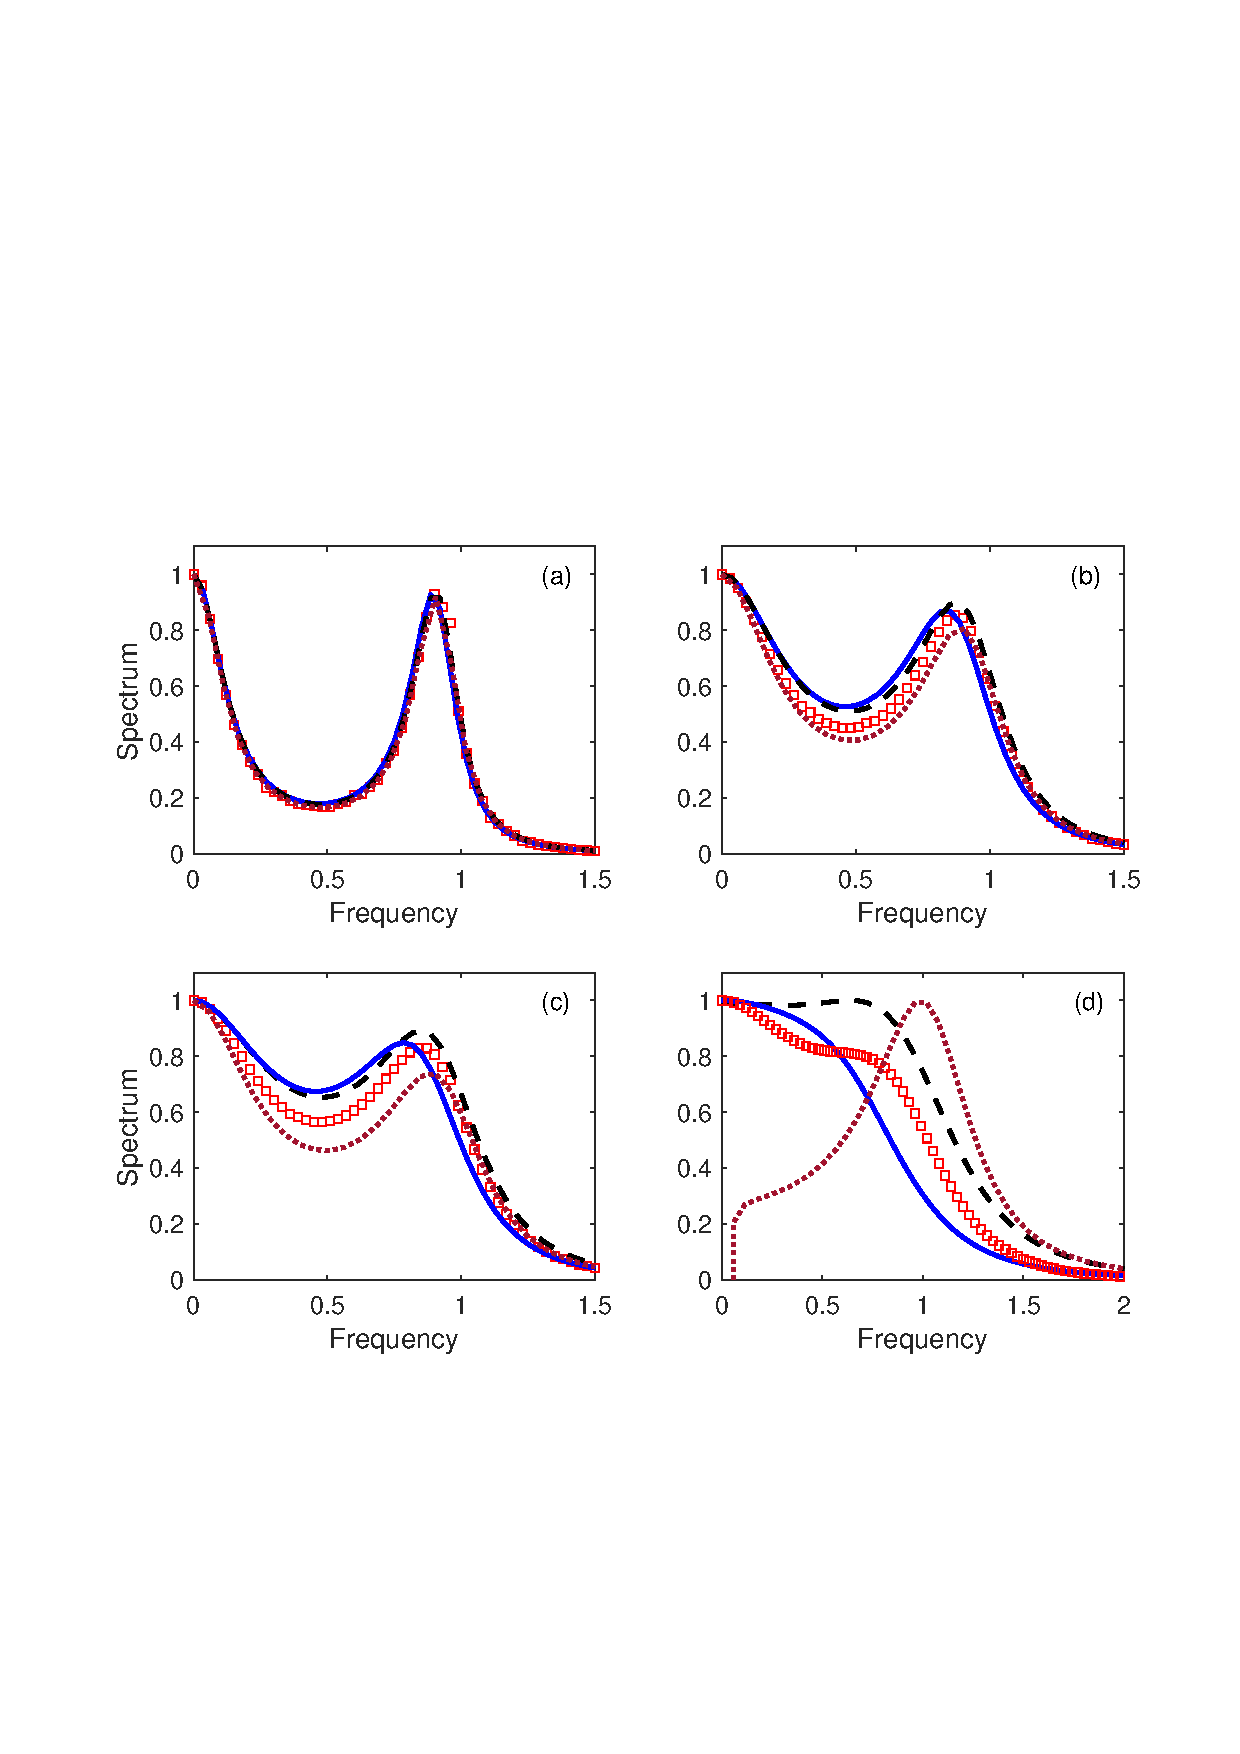
\includegraphics[width=0.7\textwidth]{FluidDynamic/IMG/s_NSBurnett.pdf}
	\caption{Spontaneous RBS spectra when (a) $\text{Kn}=0.02$, (b) $\text{Kn}=0.04$, (c) $\text{Kn}=0.05$, and (d) $\text{Kn}=0.1$. Solid, dashed and dotted lines are results from the NS, Burnett and super-Burnett equations, respectively.  } % In this and subsequent figures, squares represent results from the LBE for Maxwellian gases if without specification.
	\label{fig:NSBurnett}
\end{figure}	
% Burnett equation

If the Chapman-Enskog expansion is applied to the second-order of $\text{Kn}$, the Burnett equations can be derived. For Maxwellian molecules, the linearized constitutive relations for the stress and heat flux become
\begin{equation}
\begin{aligned}[b]
\sigma^{(B)}=\sigma^{(NS)}-\text{Kn}^2\left(\frac{4}{3}\frac{\partial^2 \rho}{\partial x^2}-\frac{2}{3}\frac{\partial^2 {T}}{\partial x^2}\right),\\
q^{(B)}=q^{(NS)}-\frac{7}{4}\text{Kn}^2\frac{\partial^2u}{\partial x^2}.
\end{aligned}
\end{equation}	
\index{Chapman-Enskog expansions!Burnett equation}
\index{Chapman-Enskog expansions!Super-Burnett equation}



The super-Burnett equations can be derived if the Chapman-Enskog expansion is applied to the third-order of $\text{Kn}$, where the stress and heat flux in this particular problem are~\cite{Shavaliyev1993}:
\begin{equation}\label{SB}
\begin{aligned}[b]
\sigma^{(SB)}=\sigma^{(B)}+\frac{2}{9}\text{Kn}^3\frac{\partial^3 u}{\partial x^3},\\
q^{(SB)}=q^{(B)}+\text{Kn}^3\left(\theta_7\frac{\partial^3T}{\partial x^3}-\frac{5}{8}\frac{\partial^3\rho}{\partial x^3}\right),
\end{aligned}
\end{equation}
with $\theta_7=-{157}/{16}$ for Maxwellian molecules. 


%Like the Burnett equations, the super-Burnett equations are  unstable to disturbance with small wavelength. Zhong \textit{et al.} proposed the augmented Burnett equations~\cite{Zhong1993}. They kept the nonlinear expressions for the stress and heat flux from the Burnett equations at the second order of $\text{Kn}$, while the third-order parts are chosen from the super-Burnett equations as the corresponding linearized terms in one-dimensional problem. In this Rayleigh-Brillouin scattering problem, expressions for the stress and heat flux in the augmented Burnett equations are also given by Eq.~\eqref{SB}. The coefficient $\theta_7$, however, is chosen as $\theta_7=11/16$, due to the wrong calculation in Ref.~\cite{WCS1982}; this erroneous parameter happens to make the augmented Burnett equations stable.


Figure~\ref{fig:NSBurnett} shows the spectra of spontaneous RBS. It is seen that the NSF equations perform well up to $\text{Kn}\approx0.02$. The Burnett equations, although accurate to the second-order of $\text{Kn}$, seems do not improve the accuracy in predicting the spectra of spontaneous RBS. It is surprising that the super-Burnett equations derived to the third-order of $\text{Kn}$ in the Chapman-Enskog expansion perform much worse than the Burnett equations that are obtained from the Chapman-Enskog expansion to the second-order of $\text{Kn}$, especially when $\text{Kn}=0.1$. This conforms the criticism that one does not know what step of the approximation is required or sufficient to obtain a solution that is correct up to order $\text{Kn}^n$~\cite{Cercignanibook1988,Sone2002Book}. 




\subsubsection{Moment equations}
\index{moment equations}
\index{moment equations!Grad 13}

%Moment equations are derived through the method of ansatz, that is, the VDF $f(t,\bm{x},\bm{v})$ in the Boltzmann equation is assumed to be the product of Gaussian function and several low-order Hermite polynomials with the coefficients related to the moments of VDF. 

%The first set of moment equations obtained by Grad~\cite{Grad1949} consists of 13 macroscopic quantities, where the distribution function is given by Eq.~\eqref{Grad13VDF}. 

In Rayleigh-Brillouin scattering the stress and heat flux in the G13 equations satisfy the following equations:
\begin{equation}\label{G13}
\begin{aligned}[b]
\frac{\partial \sigma}{\partial t}+\frac{4}{3}\frac{\partial u}{\partial x}+\frac{8}{15}\frac{\partial q}{\partial x}=-\frac{\sigma}{\text{Kn}},\\
\frac{\partial q}{\partial t}+\frac{\partial \sigma}{\partial x}+\frac{5}{2}\frac{\partial {T}}{\partial x}=-\frac{2}{3}\frac{q}{\text{Kn}}.
\end{aligned}
\end{equation}

The spectrum of spontaneous RBS can be obtained by solving the following matrix:
\begin{equation}\label{Grad_sp}
\left[ \begin {array}{cccccc} 
-i\varpi&2i\pi&0 &0 &0
\\ \noalign{\medskip}
2i\pi&-i\varpi &2i\pi &2i\pi &0
\\ \noalign{\medskip}
0&2\,i\pi&-\frac{3}{2}i\varpi &0 &2i\pi
\\ \noalign{\medskip}
0  &\frac{8}{3}i\pi  & 0 &-i\varpi+\frac{1}{\text{Kn}}  &\frac{16}{15}i\pi
\\ \noalign{\medskip}
0  & 0 & 5i\varpi &2i\varpi  &-i\varpi+\frac{2}{3\text{Kn}}
\end {array} \right]
\left[ \begin {array}{cccccc} \hat\rho \\ \hat{u}
\\ \hat{T}  \\ \hat\sigma \\ \hat{q}
\end {array} \right] =
\left[ \begin {array}{cccc} 1\\ 0
\\ 0 \\0 \\0
\end {array} \right], 
\end{equation}	
where $\hat{\sigma}$ and $\hat{q}$ are respectively the Laplace-Fourier transform of $\sigma$ and $q$ in the temporal-spatial domains.
%where the analytical solutions are too complicated and hence are not shown.

%\begin{figure}
%	\centering
%	\includegraphics[scale=0.55,viewport=80 20 740 370,clip=true]{Moment2.eps}
%	\caption{Spectra of the spontaneous (top row) and coherent (bottom row) RBS. The horizontal and vertical axis are the normalized frequency and spectrum, respectively. Form the left to right, the Knudsen number in each column are 0.04, 0.06, 0.08, and 0.1, respectively. Solid, dashed, and dotted lines are the results from the G13, R13, and R26 moment equations, respectively. Triangles and solid circles are results from Eu's generalized hydrodynamic equations and coupled constitutive relations~\eqref{CCR}, respectively.  }
%	\label{fig:moment}
%\end{figure}


\begin{figure}[t]
	\centering
	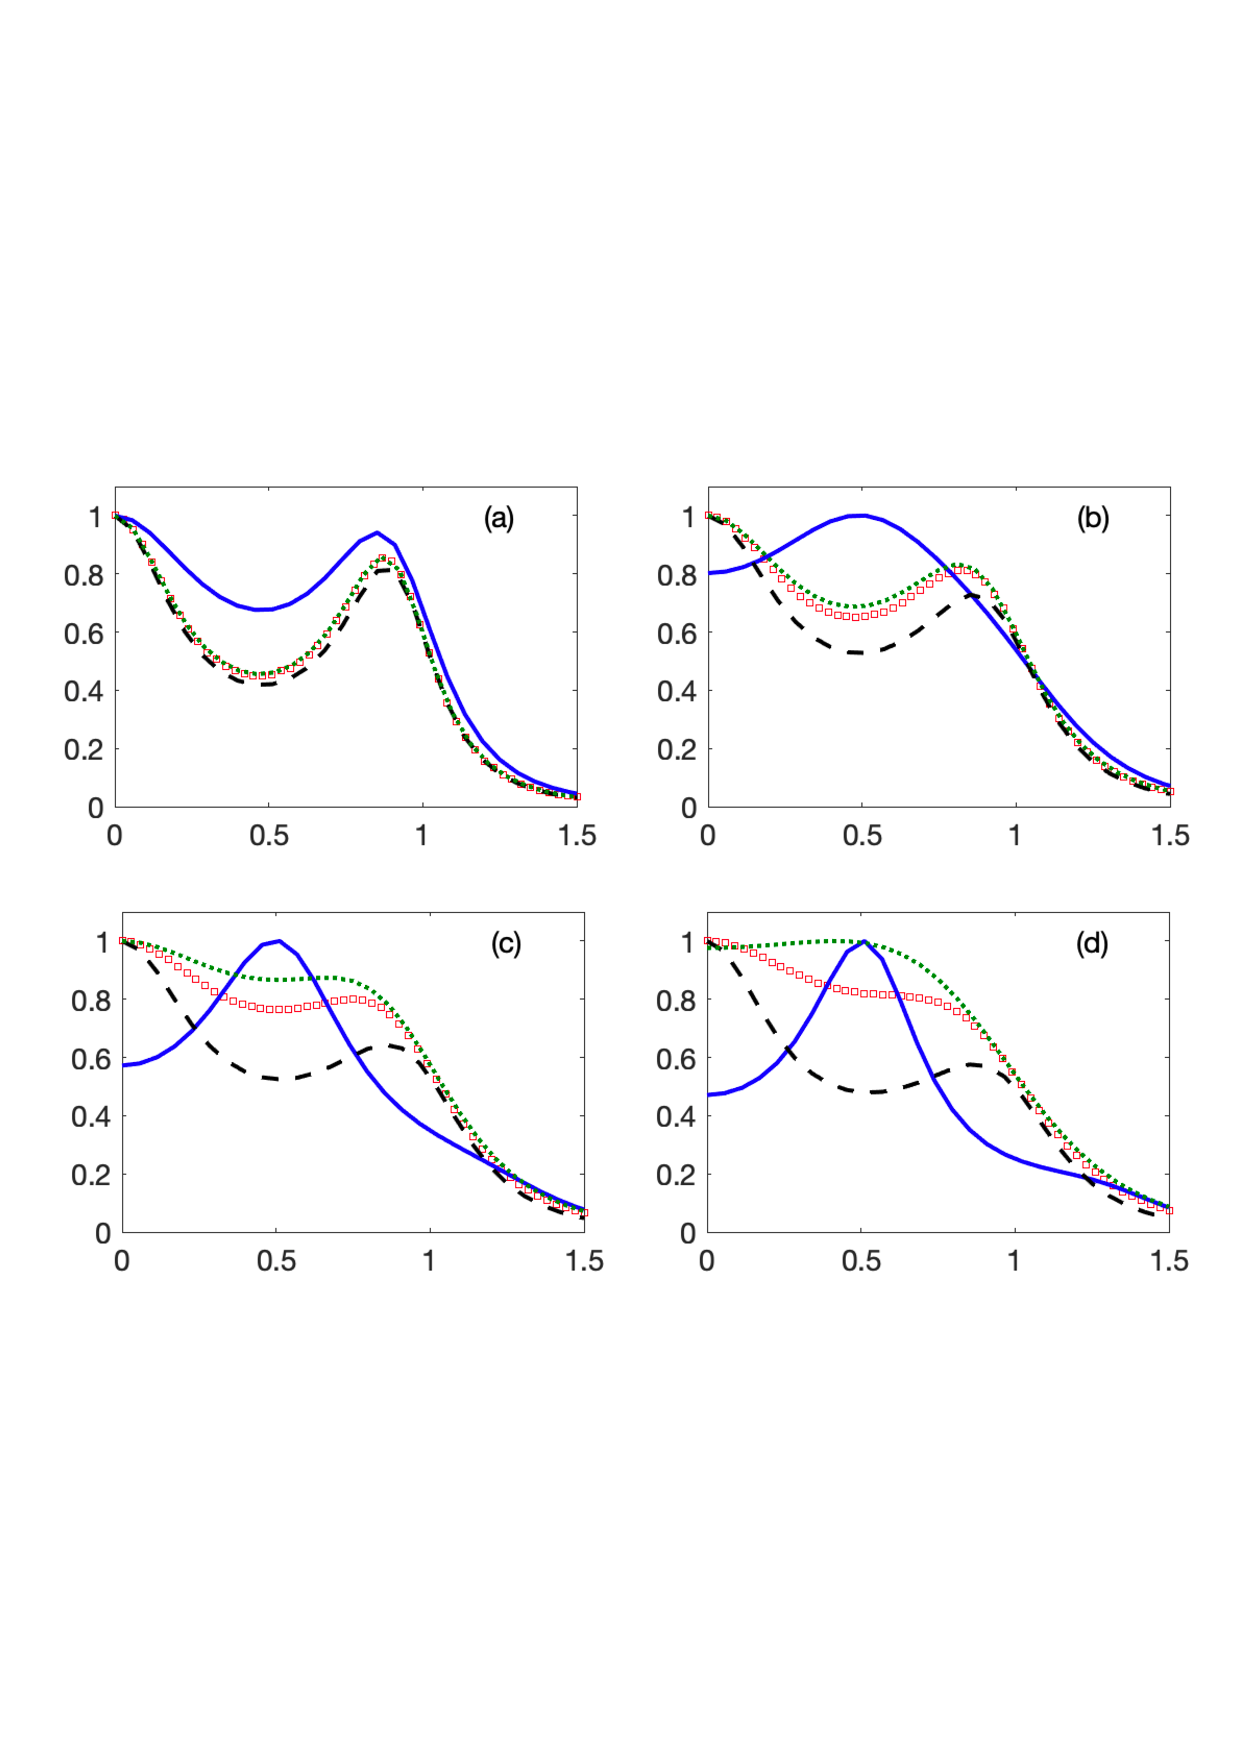
\includegraphics[scale=0.6]{FluidDynamic/IMG/Moment.pdf}
	\caption{Spectra of the spontaneous RBS. The horizontal and vertical axis are the normalized frequency and spectrum, respectively. Form the left to right, the Knudsen numbers in each column are 0.04, 0.06, 0.08, and 0.1, respectively. Solid, dashed, and dotted lines are the results from the G13, R13, and R26 moment equations, respectively.  }
	\label{fig:moment}
\end{figure}


\index{moment equations!Regularized 13}

Note that the G13 equations are accurate to the second-order of $\text{Kn}$, which have been extended to the R13 equations that are accurate to the third-order of $\text{Kn}$~\cite{henning}. The governing equations for the stress and heat flux become
\begin{equation}
\begin{aligned}[b]
\frac{\partial \sigma}{\partial t}+\frac{4}{3}\frac{\partial u}{\partial x}+\frac{8}{15}\frac{\partial q}{\partial x}-\frac{6}{5}\text{Kn}\frac{\partial^2\sigma}{\partial x^2}=-\frac{\sigma}{\text{Kn}},\\
\frac{\partial q}{\partial t}+\frac{\partial \sigma}{\partial x}+\frac{5}{2}\frac{\partial {T}}{\partial x}-\frac{18}{5}\text{Kn}\frac{\partial^2q}{\partial x^2}=-\frac{2}{3}\frac{q}{\text{Kn}}.
\end{aligned}
\end{equation}


Similarly, the evolution of the stress and heat flux in the linearized R26 equations, which are accurate up to the fifth-order of $\text{Kn}$, are governed by~\cite{Gu2009JFM}:
\begin{equation}
\begin{aligned}[b]
\frac{\partial \sigma}{\partial t}+\frac{4}{3}\frac{\partial u}{\partial x}+\frac{8}{15}\frac{\partial q}{\partial x}+\frac{\partial \bar{m}}{\partial x}=-\frac{\sigma}{\text{Kn}},\\
\frac{\partial q}{\partial t}+\frac{5}{2}\frac{\partial {T}}{\partial x}+\frac{\partial \sigma}{\partial x}+\frac{1}{6}\frac{\partial\bar{\Delta}}{\partial{}x}+\frac{1}{2}\frac{\partial\bar{R}}{\partial{x}}=-\frac{2}{3}\frac{q}{\text{Kn}},
\end{aligned}
\end{equation}
where the higher-order moments $\bar{m}$, $\bar{\Delta}$, and $\bar{R}$ are governed by the following equations:
\begin{equation}\label{Gu_R26}
\begin{aligned}[b]
\frac{\partial\bar{m}}{\partial{t}}+\frac{9}{5}\frac{\partial\sigma}{\partial{x}}+\frac{9}{35}\frac{\partial\bar{R}}{\partial{x}}-\frac{16}{7}\frac{\text{Kn}}{A_{\phi1}}\frac{\partial^2\bar{m}}{\partial{x}^2}=-\frac{3}{2}\frac{\bar{m}}{\text{Kn}},\\
\frac{\partial\bar{\Delta}}{\partial{t}}+8\frac{\partial{q}}{\partial{x}}-\frac{7\text{Kn}}{3}\frac{\partial^2\bar{\Delta}}{\partial{x}^2}-4\text{Kn}\frac{\partial^2\bar{R}}{\partial{x^2}}=-\frac{2}{3}\frac{\bar{\Delta}}{\text{Kn}},\\
\frac{\partial\bar{R}}{\partial{t}}+\frac{56}{15}\frac{\partial{q}}{\partial{x}}+2\frac{\partial\bar{m}}{\partial{x}}-\frac{\text{Kn}}{5}\left(\frac{54}{7A_{\psi1}}+\frac{16}{3}\right)\frac{\partial^2\bar{R}}{\partial{x}^2}-\frac{28\text{Kn}}{45}\frac{\partial^2\bar{\Delta}}{\partial{x}^2}=-\frac{7}{6}\frac{\bar{R}}{\text{Kn}},
\end{aligned}
\end{equation}
with $A_{\phi1}=2.097$ and $A_{\psi1}=1.698$.

\index{moment equations!Regularized 26}

Figure~\ref{fig:moment} shows the RBS spectra obtained from the G13, R13, and R26 moment equations. When $\text{Kn}=0.02$, all the moment equations predict the same spectrum as that from the LBE. However, even when $\text{Kn}$ is increased to $\text{Kn}=0.04$, spectra predicted by the G13 equations deviate significantly from those of the LBE. The R13 equations are accurate up to $\text{Kn}\approx0.04$, while the R26 equations are accurate up to $\text{Kn}\approx0.06$. 

%Interestingly,  we accidentally changed the value of $A_{\psi1}$ to $-1.698$, and found that excellent agreement is achieved for Knudsen number up to $0.1$ for both spontaneous and coherent RBS.

%Overall, the accuracy of the R26  equations are worse than the augmented Burnett equation with $\theta_7=-60/16$. 

%It should be noted that Gu has also derived the regularized 35 moment equations, where the distribution function is expanded to the fifth-order polynomials and all the relevant moments are included. For the 1D Rayleigh-Brillouin scattering problem, only one extra equation for the higher-order moment is added:
%\begin{equation}
%\frac{\partial \bar\phi}{\partial{t}}+\frac{16}{7}\frac{\partial \bar{m}}{\partial{x}}-\frac{96\text{Kn}}{245A_{\psi1}}\frac{\partial^2 \bar{R}}{\partial{x}^2}-\frac{25\text{Kn}}{9A_{w1}}\frac{\partial^2\bar\phi}{\partial{x}^2}=-\frac{A_{\phi1}}{\text{Kn}}\bar{\phi},
%\end{equation}
%with $A_{w1}=2.743$ for Maxwellian molecules, while the equation for $\bar{m}$ in~\eqref{Gu_R26} is replaced by
%\begin{equation}
%\frac{\partial\bar{m}}{\partial{t}}+\frac{9}{5}\frac{\partial\sigma}{\partial{x}}+\frac{9}{35}\frac{\partial\bar{R}}{\partial{x}}+\frac{\partial\bar{\phi}}{\partial{x}}=-\frac{3}{2}\frac{\bar{m}}{\text{Kn}}.
%\end{equation}
%It is noted by Gu that from 1D shear flow the R35 equations are better than the R26 equations, but not much. The same conclusion can be made in the Rayleigh-Brillouin scattering problem, where the spectra from the R26 and R35 equations are nearly identical, since there are both accurate to $O(\text{Kn}^5)$. In 2D or 3D situations, the computational costs increase as more equations are included in the system, but the accuracy is not gained proportionally. Therefore, the R26 moment equations are recommended. 






%\subsection{Rational extended thermodynamics}
%
%\begin{figure}
%	\centering
%	\includegraphics[scale=0.5,viewport=0 0 660 290,clip=true]{PRL.eps}
%	\caption{Comparisons in the spectra of spontaneous RBS between the experimental data (the solid line) by Greytak \& Benedek~\cite{Greytak1966PRL}, the LBE (the dashed line) for polyatomic gas~\cite{Wu2015JFM}, and the rational extended thermodynamics with 14 moments (the dash-dotted line) by Ruggeri \& Sugiyama~\cite{Ruggeri2015Book}. The light is scattered from CO$_2$ when $\text{Kn}=0.1114$. Note that the frequency is normalized by 1.06~GHz, and the shown spectra are the convolution of $S_s(Kn,f_s)$ and the Lorentzian function $Lor(f_s)$ with the Full Width at Half Maximum being 210~MHz, i.e.,  $Lor(f_s)\propto1/(f_s^2+9.8\times10^{-3})$.   }
%	\label{fig:PRL}
%\end{figure}
%
%
%
%Rational extended thermodynamic equations for rarefied gas dynamics are derived from the gas kinetic equation in a manner similar to the derivation of moment equations, but the distribution function is instead obtained by the maximum entropy principle. Recently, it has been used to study the spontaneous RBS spectra in polyatomic gases by considering only 14 moments (i.e. in addition to the 13 moments in the G13 equations, the dynamical pressure that is related to the bulk viscosity is also considered); the corresponding macroscopic equations can be found in the Chapter 9 of the book by Ruggeri \& Sugiyama~\cite{Ruggeri2015Book}, which degenerate to the G13 equations for monatomic gases when the deviation from equilibrium is weak. 
%
%
%The spectrum of spontaneous RBS from the rational extended thermodynamics with 14 moments has been compared with the experiment~\cite{Greytak1966PRL}, where the light with the effective wave vector $k=1.98\times10^{5}$~cm$^{-1}$ is scattered by CO$_2$ at a temperature 298~K and pressure 750~mm~Hg. In the numerical calculation of the spectrum of spontaneous RBS based on the LBE for polyatomic gas, we use the method developed in Ref.~\cite{Wu2015JFM}, with the ratio of the bulk viscosity to the shear viscosity of CO$_2$ being 0.39~\cite{Gu2014OL}. From Fig.~\eqref{fig:PRL} we can find the huge difference between the results of rational extended thermodynamics and experiment, while our LBE solution gives a good prediction of the RBS spectrum. We conclude that the accuracy of the rational extended thermodynamics is roughly at the same order with the G13 equations.



\subsubsection{Discussions}\label{Conclusions}

%The accuracy of macroscopic equations is summarized and visualized more clearly in %Fig.~\ref{fig:compare}, where the relative difference in the RBS spectra is shown as a function of the Knudsen number. The solution may be viewed being accurate when the relative difference is less than 0.05. It should be noted that in Rayleigh-Brillouin scattering both the spatial and temporal Knudsen numbers play important roles. For steady-state problems, the range of applicability of these macroscopic equations may move to larger values of $\text{Kn}$.  

Based on the benchmarking solutions from the Boltzmann equation for the spectra of Rayleigh-Brillouin scattering, we have assessed the accuracy of macroscopic equations. Interestingly, as the order of Chapman-Enskog expansion increases, the accuracy of the obtained macroscopic equations does not necessarily increase (say, when $\text{Kn}\gtrapprox0.03$, the super-Burnett equations are less accurate than the Burnett equations), which confirms the criticism that one does not know what step of the approximation is required or sufficient to obtain a solution that is correct up to order $\text{Kn}^n$. For the (regularized) moment equations, however, the accuracy in the prediction of RBS spectra is consistent with the accuracy in deriving these equations, that is, increases monotonically from the G13, R13, to the R26 moment equations. 

%
%\begin{figure}[t]
%	\centering
%	\includegraphics[scale=0.5]{relative_srbs}
%	\caption{
%		(left) Difference $\int_{\infty}^{\infty} |S^{LBE}-S^{Mac}| df_s$ in the spectrum of spontaneous RBS between solutions of the LBE and macroscopic equations. Note that before the comparison, areas of RBS spectra are normalized to unity. The solution may be viewed to be accurate when the relative difference is less than 0.05. 
%	}
%	\label{fig:compare}
%\end{figure}


%The Eu's generalized hydrodynamic equations, where the VDF contains the fourth-order Hermite polynomial, has the same level accuracy as the G13 equations, where the distribution function is expanded only up to the third-order Hermite polynomial, and it is less accurate than the R13 equations. The Brenner's bi-velocity fluid model and Dadzie's thermo-mechanically consistent Burnett equations, which contain free parameters that can not be determined from fundamental physical laws, both involve the concept of volume diffusion, do not perform well compared to the R13 equations, even when the best parameters are selected.  

\begin{figure}[t]
	\centering
	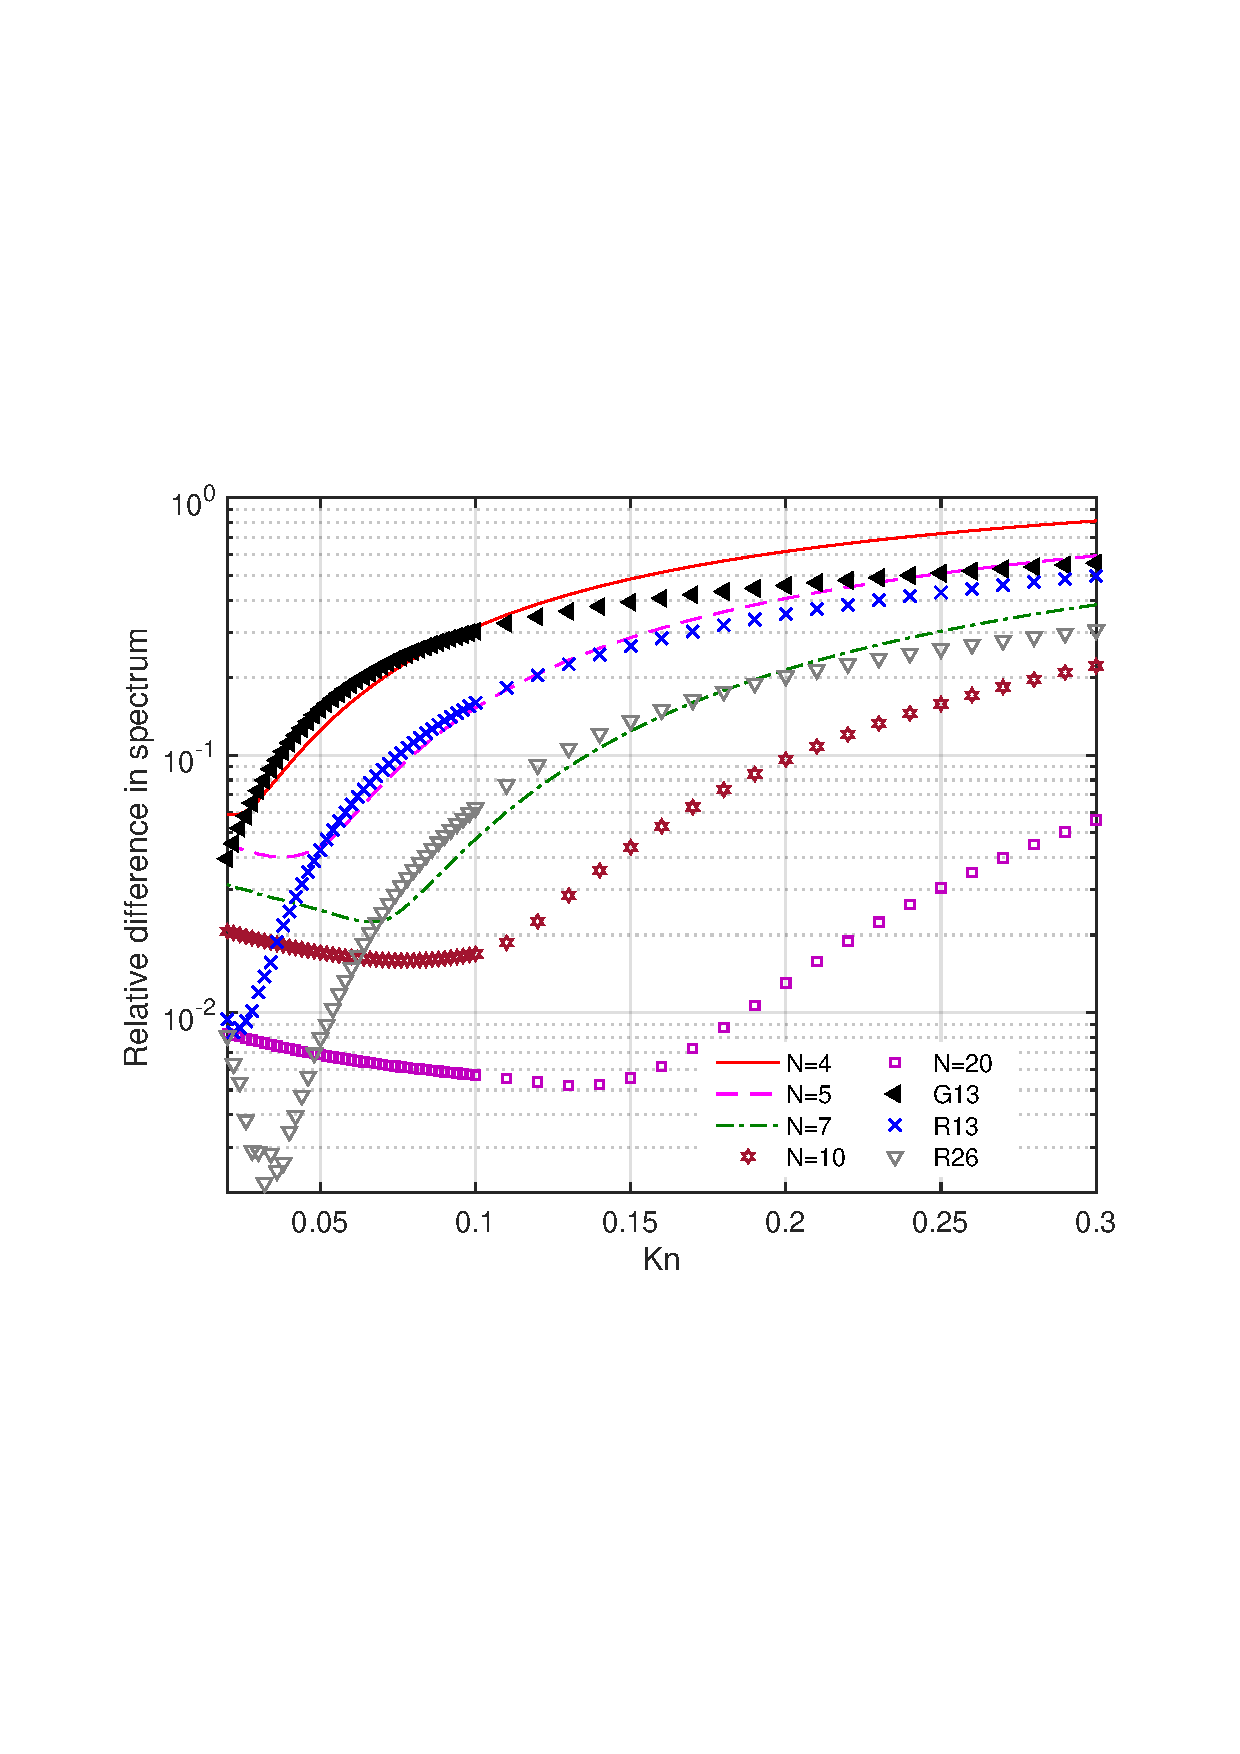
\includegraphics[scale=0.6]{FluidDynamic/IMG/compare_GH.pdf}
	\caption{Difference $\int_{\infty}^{\infty} |S^{LBE}-S_{GH}^{N}| df_s$ in the spectrum of spontaneous RBS, where $S_{GH}^{N}$ is the spectrum obtained by solving the Shakhov kinetic model in section~\ref{shakhov_model_chapter} with the Gauss-Hermite quadrature of order $N$.  Note that before the comparison, areas of RBS spectra are normalized to unity. The solution may be viewed being accurate when the relative difference is less than 0.05. Also note that the relative difference when $N=5, 7, 10$ and 20 does not decrease with $\text{Kn}$ when $\text{Kn}\lesssim0.1$ is probably because the spectrum between the Rayleigh and Brillouin peaks is nearly zero [see Fig.~\ref{fig:RBS_demo}] so any tiny difference is magnified.}
	\label{fig:compare2}
	% in the three-dimensional molecular velocity space $\bm{v}$, the number of total discrete velocity points is $N^3$; note that the corresponding Grad moment equations have $(N+1)(N+2)(N+3)/6$ moments~\cite{FanThesis}.
\end{figure}

From these comparisons, it may be concluded that the regularized moment method is a proper way to derive higher-order macroscopic equations to describe the rarefied gas dynamics, where the derivation is straightforward, and its accuracy is definitive and controllable, that is, the accuracy increases with the number of moments or order of Hermite polynomials used to approximate the VDF. This is quite important in numerical simulations, where the error may be estimated in prior. To further illustrate this point, we study the performance of higher-order moment method, by solving the linearized Shakhov equation numerically using the discrete velocity method based on the Gauss-Hermite quadrature~\cite{Shakhov_S}, which is equivalent to the Grad moment method at different order of approximations~\cite{Shan2006JFM}. To be specific, if the $N$-th order Gauss-Hermite quadrature is considered in the discretization of molecular velocity space, the moment up to the order $N-1$ can be captured accurately~\cite{Shan2006JFM}. Consider the fact that the G13 equations where the distribution function is expanded up to third-order Hermite polynomials are accurate to $O(\text{Kn}^2)$, the numerical solution of the Shakhov equation based on the Gauss-Hermite quadrature of order $N$ has an accuracy of $O(\text{Kn}^{N-2})$.






%\cite{Shakhov1968,Shakhov_S,Shakhov1974}:
%\begin{equation}\label{Shakhov_RBS}
%\begin{aligned}[b]
%\frac{\partial h}{\partial t}+v_1\frac{\partial h}{\partial x_1}=\frac{\delta_{rp}}{\pi^{3/2}}\exp(-v^2)
%\left[\varrho+2u_1v_1+T\left(v^2-\frac{3}{2}\right)+\frac{4}{15}q_1v_1\left(v^2-\frac{5}{2}\right)\right]
%-\delta_{rp}h,
%\end{aligned}
%\end{equation}
%where
%$\varrho=\int{h}\mathrm{d}\bm{v}$ is the perturbed number density, $u_1=\int v_1{h}\mathrm{d}\bm{v}$ is the perturbed velocity,  $T=\frac{2}{3}\int{}v^2{h}\mathrm{d}\bm{v}-\rho$ is the perturbed temperature, and $q_1=\int{}v^2v_1{h}\mathrm{d}\bm{v}-\frac{5}{2}u_1$ is the perturbed heat flux. 







Using solutions of the Shakhov model approximated by the 60th-order Gauss-Hermite quadrature as reference, we analyze the accuracy of various orders of moment equations in Fig.~\ref{fig:compare2}. We also show the relative error in the spectrum from comparisons between the G13/R13/R26 equations and the LBE. Obviously, as more moments (i.e., higher-order quadrature) are included, the accuracy increases monotonically. When $N=4$, the Gauss-Hermite quadrature yields an equivalent moment system accurate to $O(\text{Kn}^2)$, therefore, the relative difference curve almost overlaps that from the G13 equations. Similarly, $N=5$ and 7 yield equivalent moment systems accurate to $O(\text{Kn}^3)$ and $O(\text{Kn}^5)$, respectively. Therefore, relative difference curves nearly overlap with those from the R13 and R26 moment equations in a wide range of Knudsen numbers.


It can also be seen from Fig.~\ref{fig:compare2} that at large values of $\text{Kn}$ the convergence rate of moment equations is slow. For example, when $\text{Kn}=0.3$, when $N$ is increased from 5 to 20, that is, when the accuracy of the equivalent moment systems is increased from $O(\text{Kn}^3)$ to $O(\text{Kn}^{18})$, the error is only reduced by about one order of magnitude. And the solution of $N=20$ can be marginally viewed as accurate. Accuracy of moment systems may become worse in wall-bounded problems such as the Poiseuille flow between two parallel plates~\cite{Su2007PRE}, as Gauss-Hermite polynomials are not good at capturing the discontinuities in VDF. 


To conclude, higher-order Chapman-Enskog expansion does not necessarily lead to more accurate prediction of rarefied gas dynamics, while the moment method produces more accurate results when more moments are included, but the convergence to true solutions may be slow when the Knudsen number is large. 

%This research would shed some light on how to choose/develop macroscopic equations for rarefied gas dynamics. % After all, knowing history helps advance future without past mistakes.      









\section{Convergence speed of moment equations}\label{sound_section}
\index{sound wave}

We now assess the accuracy of macroscopic equations in the problem of sound propagation in gas confined between the transducer and receiver~\cite{Wu2020AIA}, see Fig.~\ref{fig:sound}. We use the linearized Shakhov kinetic model equation, as the Gauss-Hermite quadrature can be applied~\citep{Shan2006JFM} to mimic the behavior of moment equations at any order, replacing the complicated derivation and solving of high-order moment equations beyond R26; the numerical method is given in Section~\ref{sound_gsis_1D}, where the numerical solution agrees well with  experimental data of Schotter~\cite{Schotter1974}, see Fig.~\ref{fig:sound}.


Macroscopic equations are the same as in the Rayleigh-Brillouin scattering problem, except for the R26 equations we have $A_M=1=A_{\Delta1}=A_{\Omega1}=A_{\phi1}=A_{\psi1}=A_{R1}=1$ in Eq.~\eqref{Gu_R26}, as derived from the Shakhov kinetic model. The boundary conditions for NS and R13 equations corresponding to the diffuse boundary condition for gas kinetic model equations can be found in Ref.~\cite{Struchtrup2011}, while that for R26 equations is given in Ref.~\cite{Gu2009JFM}.



\begin{figure}[t]
	\centering
	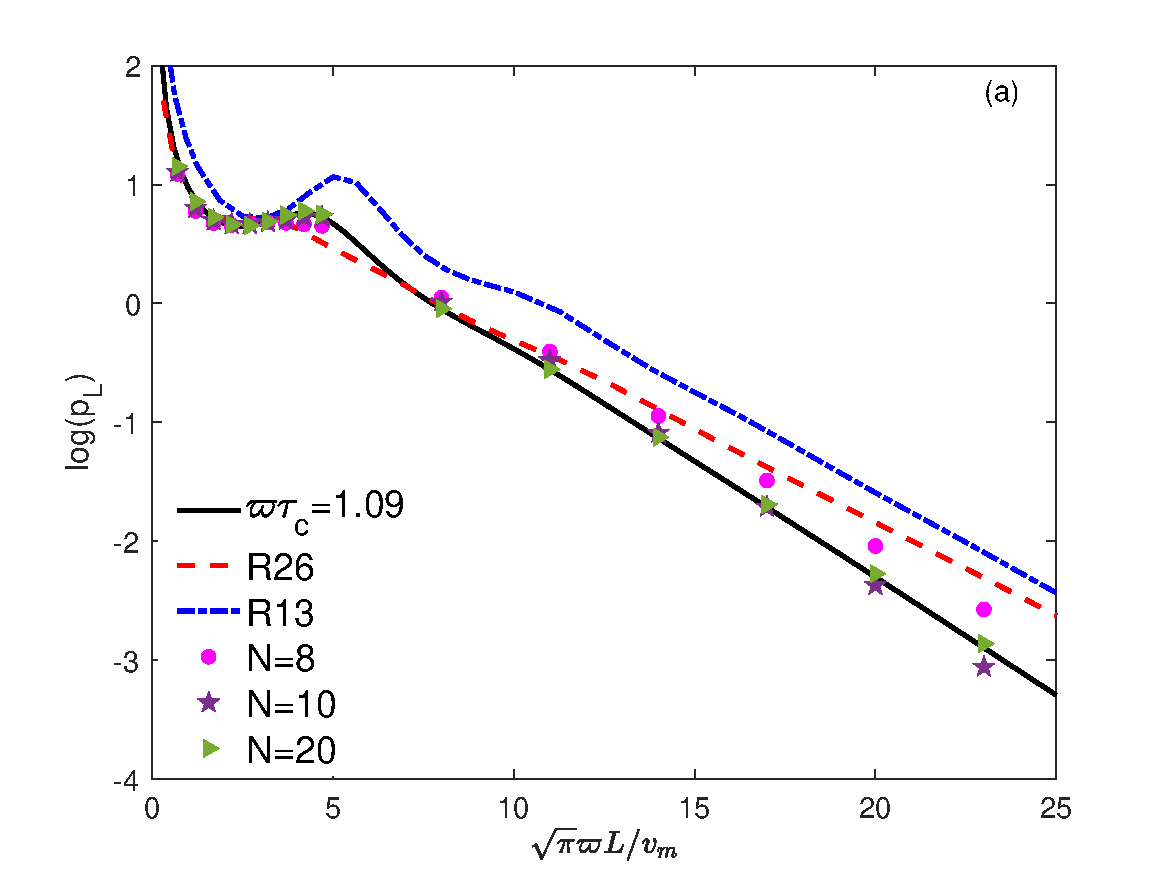
\includegraphics[width=0.49\textwidth]{FluidDynamic/IMG/testOmgTau1_09Copy.pdf}
	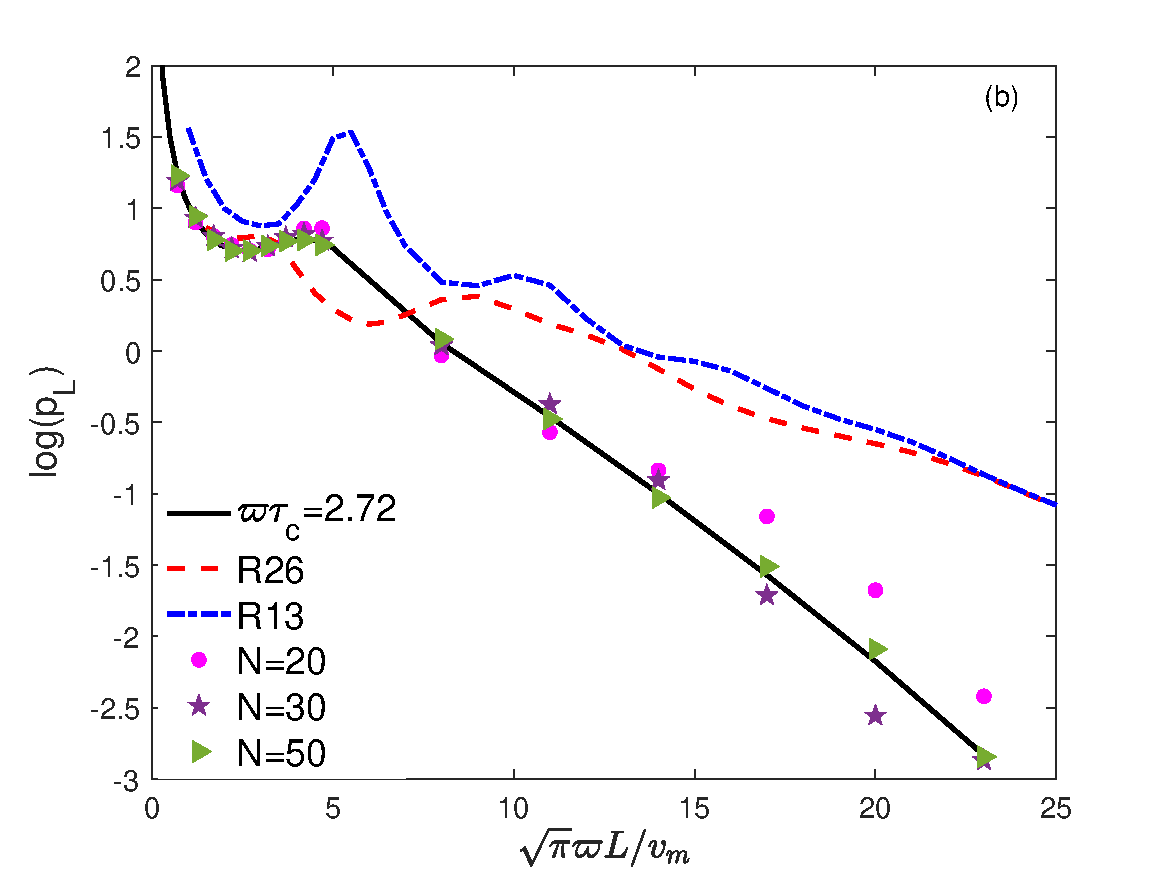
\includegraphics[width=0.49\textwidth]{FluidDynamic/IMG/testOmgTau2_72.pdf} 
	\caption{ Convergence test of moment equations: sound amplitude at the receiver as function of the dimensionless length $\sqrt\pi\varpi{L}/v_m$. Solid lines represent the accurate results from the Shakhov model solved by the discrete velocity method~\citep{SuArXiv2019}. Symbols are approximate solutions of the Shakhov model when the molecular velocity space $\bm{v}$ is discretized according to Gauss-Hermite quadrature of order $N$; these solutions are equivalent to those of Grad moment equations (having $(N+1)(N+2)(N+3)/6$ moments) that are accurate up to the order of $\text{Kn}^{N-2}$.  }
	\label{fig:sound_convergence}
\end{figure}


The parameter $\varpi{\tau_c}$ in Fig.~\ref{fig:sound} is proportional to the temporal Knudsen number $\text{Kn}_t$ as $\varpi{\tau_c}=2\sqrt{2}\pi\text{Kn}_t$. Therefore, as $\varpi{\tau_c}$ increases, the rarefaction effects become stronger, so macroscopic equations gradually lose accuracy. The NSF equations are accurate when $\varpi{\tau_c}=0.1$ (not shown), but are already very inaccurate when $\varpi{\tau_c}=0.3$; R13 equations, which are accurate to the order of $\text{Kn}^3$, give reasonable good results up to $\varpi{\tau_c}=0.3$, see  Fig.~\ref{fig:sound}. While R26 equations, which are accurate to the order of $\text{Kn}^5$, predict the normal pressure at the receiver fairly well up to $\varpi\tau_c=0.67$. This finding is in agreement with that in the spontaneous RBS, i.e., the accuracy of moment equations increases when more moments are included in macroscopic equations.  





%\subsubsection{Reason of slow convergence of moment systems}
%\index{Slow convergence}
\index{moment equations}

Now we consider the speed of convergence of moment systems for moderate and highly rarefied gas flows, that is, we are interested in how many moments should be included to give reasonable prediction of sound pressure. %Since the derivation and solving of higher-order moment system is extremely difficult, we solve the Shakhov model using the Gauss-Hermite quadrature of order $N$ instead; this is equivalent to the Grad moment equations where the VDF is expanded by Hermite polynomials up to $N$-th order. 



\index{velocity distribution function}
\begin{figure}[t]
	\centering
	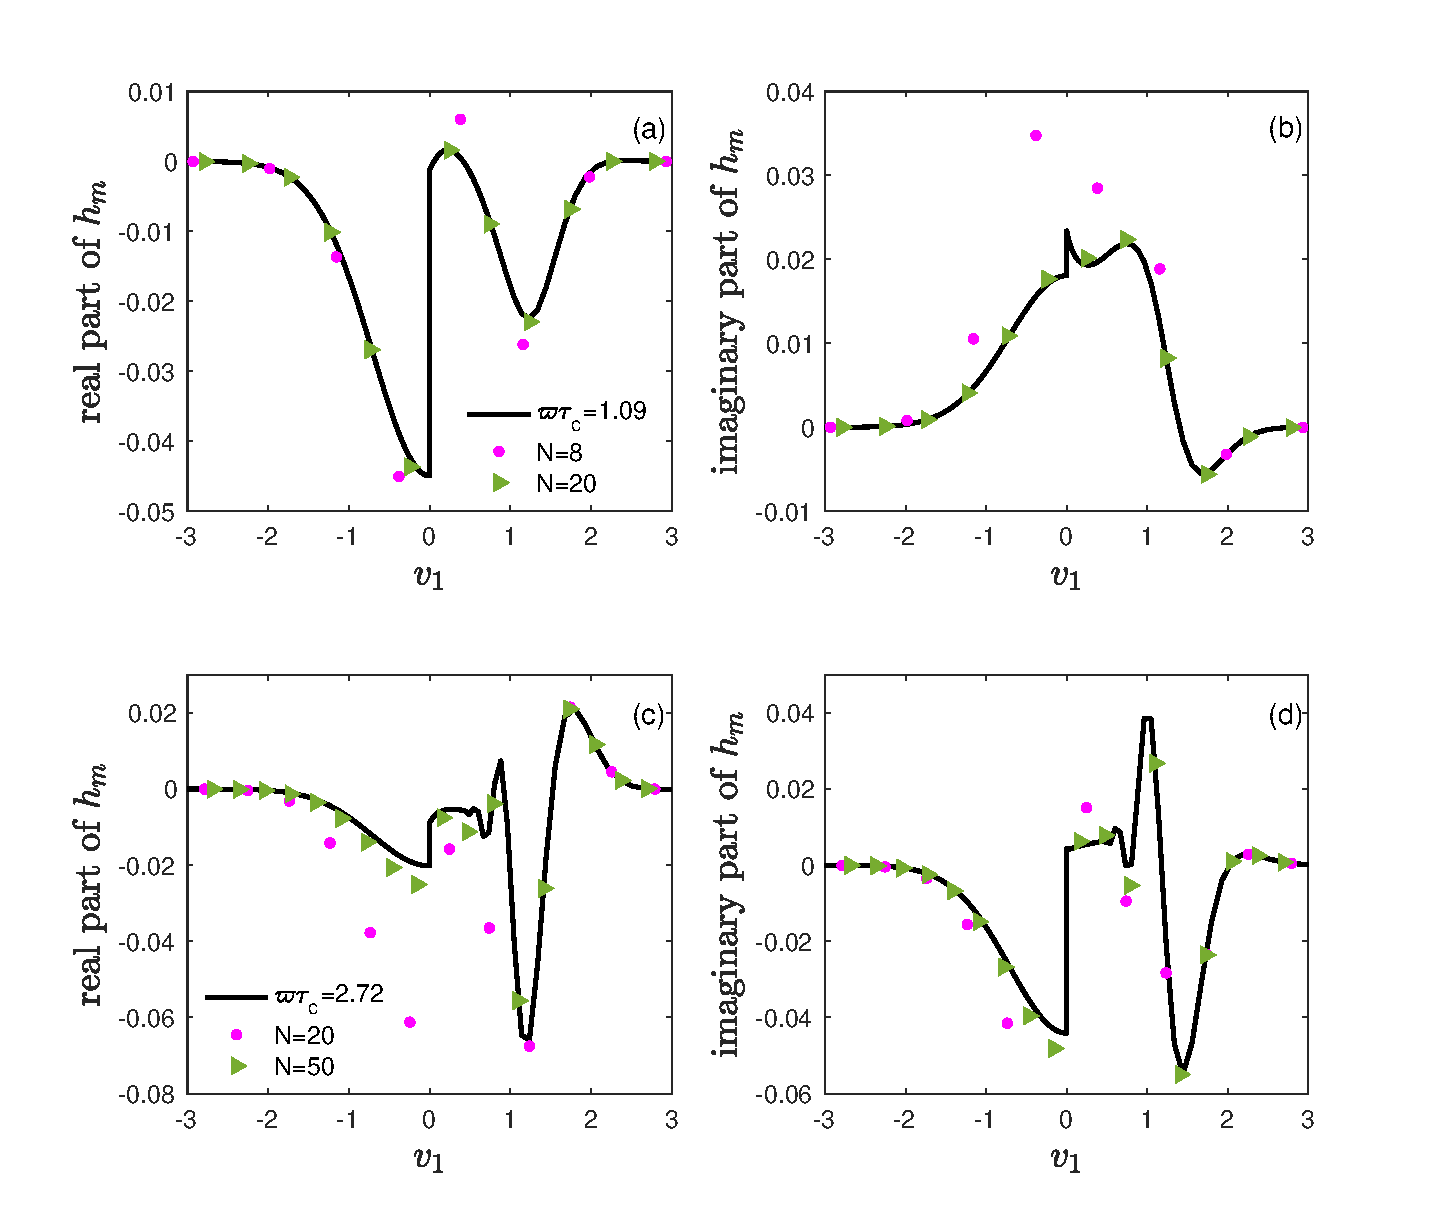
\includegraphics[width=0.8\textwidth]{FluidDynamic/IMG/vdf_sound.pdf}
	\caption{\index{velocity distribution function!marginal} Marginal VDF at the receiver. (a, b) $\varpi{\tau_c}=1.09$ and (c,d) $\varpi{\tau_c}=2.72$. In both cases, $\sqrt{\pi}\varpi{L}/v_m=20$. Solid lines represent the accurate results from the Shakhov model solved by the discrete velocity method~\citep{SuArXiv2019}, while symbols are approximate solutions of the Shakhov model when the molecular velocity space $\bm{v}$ is discretized by the Gauss-Hermite quadrature of order $N$.  }
	\label{fig:vdf_sound_convergence}
\end{figure}

Typical results are depicted in Fig.~\ref{fig:sound_convergence}. When $\varpi\tau_c=1.09$, the result of using Gauss-Hermite quadrature of order 8 is more accurate than that of R26 equations. This is because $N=8$ corresponding to Grad moment equations of accuracy $O(\text{Kn}^6)$, one order more accurate than R26 equations. In order to obtain accurate results, however, the VDF has to be expanded into Hermite polynomials to the $20$-th order. We say the convergence is rather slow as increasing $N$ from 10 to 20 only results in marginal improvement of accuracy. This situation becomes more severe when $\varpi\tau_c$ increases to 2.72. From Fig.~\ref{fig:sound_convergence}(b) we see that R13 and R26 moments equations are quite inaccurate; in order to have accurate results, Gauss-Hermite quadrature of order higher than 50 is needed.


The slow convergence of moment systems in describing rarefied gas flows may be explained at the mesoscopic level. To this end we note that when the steady oscillation is reached,  the derivation VDF $f-F_{eq}$ is proportional to the real part of $\exp(i\varpi{t})h(x_1,\bm{v})$. The marginal VDF $h_{m}=\iint{hdv_2v_3}$ at the resting receiver is plotted in Fig.~\ref{fig:vdf_sound_convergence}. When $\varpi\tau_c=1.09$, the spatial and temporal Knudsen numbers are respectively $\text{Kn}=0.069$ and $\text{Kn}_t=0.123$, the VDF is smooth, except it has a huge jump at $v_1=0$. This kind of jump (discontinuities) is typical in wall-bounded rarefied gas flows. The VDF when $v_1<0$ is described by the Gaussian function as per Maxwell's diffuse boundary condition, while that at $v_1>0$ deviates from the equilibrium distribution because of the relative large value of $\text{Kn}_t$ so that the system does not have enough time to reach equilibrium. The Gauss-Hermite quadrature of order $N=8$ cannot predict the gas pressure in Fig.~\ref{fig:sound_convergence}(a) because the VDF in Fig.~\ref{fig:vdf_sound_convergence}(a,b), when $v_1>0$, cannot be well fitted by the Hermite polynomials up to the 8th order. Only the Gauss-Hermite quadrature of order higher than $N=20$ can give reasonable good prediction of macroscopic gas pressure at the receiver. However, from the comparison in VDF we see that this is not enough in capturing accurately the physics at the mesoscopic level. 
When $\varpi\tau_c=2.72$, the two Knudsen numbers are $\text{Kn}=0.171$ and $\text{Kn}_t=0.306$, the rarefaction effects are even stronger, and the VDF becomes more and more irregular: it not only has jump at $v_1=0$, but has rapid variations. To capture this rapid variations, the order of Gauss-Hermite quadrature needs to be very high. From the comparisons in Fig.~\ref{fig:sound_convergence}(b) and Fig.~\ref{fig:vdf_sound_convergence}(c,d) we see that although Gauss-Hermite quadrature of order $N=50$ can predict the gas pressure at the receiver, it still produces some discrepancy in the mesoscopic VDF.


Thus, the large discontinuities and rapid variations in the VDF is the underlying reason for the slow convergence of Grad moment systems, since the smooth Hermite polynomials are not good at resolving these irregular structures. In the framework of Gauss-Hermite quadrature, adding more discrete velocity grids is not economic. In highly rarefied gas flows, it is beneficial to directly solve the kinetic equation by the discrete velocity method using numerical quadratures that are more suitable for wall-bounded problems~\cite{Su2007PRE,Naris_pof,Ambrus2012PRE}, instead of deriving and solving higher-order moment systems~\cite{Cai2010Siam}. 


%In moderate and highly rarefied gas flows, it is beneficial to directly solve the kinetic model equation by the discrete velocity method using , instead of deriving and solving higher-order moment systems~\citep{Cai2010Siam}.



















